\subsection{Emulating CHERI}

Manipulating CHERI capabilities securely and correctly is a must for any CHERI-enabled emulator.
Capability encoding logic is not trivial by any means, so the \code{cheri-compressed-cap} C library was re-used rather than implementing it from scratch.
Rust has generally decent interoperability with C, but some of the particulars of this library caused issues.

\subsubsection{\code{rust-cheri-compressed-cap}}
\code{cheri-compressed-cap} provides two versions of the library by default, for 64-bit and 128-bit capabilities, which are generated from a common source through extensive use of the preprocessor.
Each variant defines a set of preprocessor macros (e.g. the widths of various fields) before including two common header files \code{cheri\_compressed\_cap\_macros.h} and \code{cheri\_compressed\_cap\_common.h}.
The latter then defines every relevant structure or function based on those preprocessor macros.
For example, a function \code{compute_base_top} is generated twice, once as  \code{cc64\_decompress\_mem} returning \code{cc64\_cap\_t} and another time as \code{cc128\_decompress\_mem} returning \code{cc128\_cap\_t}.
Elegantly capturing both sets was the main challenge for the Rust wrapper.

One of Rust's core language elements is the Trait - a set of functions and \enquote{associated types} that can be \emph{implemented} for any type.
This gives a simple way to define a consistent interface: define a trait \code{CompressedCapability} with all of the functions from \code{cheri\_compressed\_cap\_common.h}, and implement it for two empty structures \code{Cc64} and \code{Cc128}.
In the future, this would allow the Morello versions of capabilities to be added easily.
A struct \code{CcxCap<T>} is also defined which uses specific types for addresses and lengths pulled from a \code{CompressedCapability}.
For example, the 64-bit capability structure holds a 32-bit address, and the 128-bit capability a 64-bit address.

128-bit capabilities can cover a 64-bit address range, and thus can have a length of $2^{64}$.
Storing this length requires 65-bits, so all math in \code{cheri\_compressed\_cap\_common.h} uses 128-bit length values.
C doesn't have any standardized 128-bit types, but GCC and LLVM provide so-called ``extension types'' which are used instead.
Although the x86-64 ABI does specify how 128-bit values should be stored and passed as arguments\cite{specification-x86-psABI-v1.0}, these rules do not seem consistently applied\footnote{See \url{https://godbolt.org/z/qj43jssr6} for an example.}.
This causes great pain to anyone who needs to pass them across a language boundary.

Rust explicitly warns against passing 128-bit values across language boundaries, and the Clang User's Manual even states that passing \code{i128} by value is incompatible with the Microsoft x64 calling convention\footnote{\gitfile[release/13.x]{clang/docs/UsersManual.rst:3384}{llvm/llvm-project}{https://github.com/llvm/llvm-project/blob/release/13.x/clang/docs/UsersManual.rst\#x86}}.
This could be resolved through careful examination: for example, on LLVM 128-bit values are passed to functions in two 64-bit registers\footnote{\gitfile[release/13.x]{clang/lib/CodeGen/TargetInfo.cpp:2811}{llvm/llvm-project}{https://github.com/llvm/llvm-project/blob/75e33f71c2dae584b13a7d1186ae0a038ba98838/clang/lib/CodeGen/TargetInfo.cpp\#L2811}}, which could be replicated in Rust by passing two 64-bit values.
For convenience, we instead rely on the Rust and Clang compilers using compatible LLVM versions and having identical 128-bit semantics.

The CHERI-RISC-V documentation contains formal specifications of all the new CHERI instructions, expressed in the Sail architecture definition  language\footnote{\gitrepo{rems-project/sail}{https://github.com/rems-project/sail}}.
These definitions are used in the CHERI-RISC-V formal model\footnote{\gitrepo{CTSRD-CHERI/sail-cheri-riscv}{https://github.com/CTSRD-CHERI/sail-cheri-riscv}}, and require a few helper functions (see~\cite[Chapter~8.2]{TR-951}).
To make it easier to port the formal definitions directly into the emulator the \code{rust-cheri-compressed-cap} library also defines those helper functions.

The above work is available online\footnote{\redact{\gitrepo{theturboturnip/cheri-compressed-cap}{https://github.com/theturboturnip/cheri-compressed-cap}}}, and includes documentation for all C functions (which is not documented in the main repository).
That documentation is also available online\footnote{\redact{\url{https://theturboturnip.github.io/files/doc/rust_cheri_compressed_cap/}}} and partially reproduced in \cref{appx:docs:rustcherilib}.

\subsubsection{Integrating into the emulator}
% i.e. using MemoryOf trait to make all memory addressable only by capabilities
Integrating capabilities into the emulator was relatively simple thanks to the modular emulator structure.
A capability-addressed memory type was created, which wraps a simple integer-addressed memory in logic which performs the relevant capability checks.
For integer encoding mode, a further integer-addressed memory type was created where integer addresses are bundled with the DDC before passing through to a capability-addressed memory (see \cref{fig:emulatormemory}).
% For integer encoding mode, a further integer-addressed memory type was created which wraps the capability addressed mode, where all integer addresses are bundled with the DDC before passing through to the capability-addressed memory.
Similarly, a merged capability register file type was created that exposed integer-mode and capability-mode accesses.
This layered approach meant code for basic RV64I operations did not need to be modified to handle CHERI at all --- simply passing the integer-mode memory and register file would perform all relevant checks.

% i.e. isn't the module system nice for overriding specific behaviour like Capability-mode RV64I :)
Integrating capability instructions was also simple.
Two new ISA modules were created: \code{XCheri64} for the new CHERI instructions, and \code{Rv64imCapabilityMode} to override the behaviour of legacy instructions in capability-encoding-mode (see \cref{fig:module_algorithm}).
The actual Processor structure was left mostly unchanged.
Integer addresses were changed to capabilities throughout,
memory and register file types were changed as described above, and the PCC/DDC were added.

\begin{figure}
    \centering
    \begin{minipage}[c]{.4\textwidth}
      \centering
      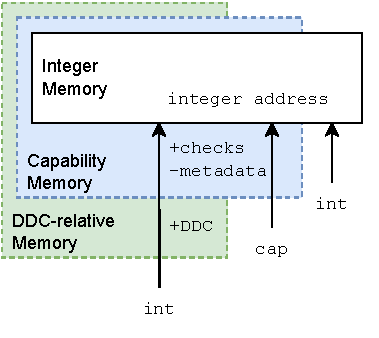
\includegraphics[width=\linewidth]{Figures/cheri_memory.pdf}
      \captionof{figure}{Emulator memory structure}
      \label{fig:emulatormemory}
    \end{minipage}\hfill%
    \begin{minipage}[c]{7.5cm}
        \centering
        {

        \small
      \begin{algorithmic}
        \If{new CHERI instruction}
            \State handle with \code{XCheri64}
        \ElsIf{basic \code{rv64} instruction}
            \If{in capability encoding mode}
                \State handle with \code{Rv64imCapabilityMode}
            \Else{}
                \State wrap memory with DDC-relative
                \State handle with \code{Rv64im}
            \EndIf{}
        \ElsIf{vector instruction}
            \If{in capability encoding mode}
                \State handle with vector unit
            \Else{}
                \State wrap memory in DDC-relative
                \State handle with vector unit
            \EndIf{}
        % \ElsIf{CSR instruction}
        %     \State handle with CSR module
        \EndIf{}
    \end{algorithmic}
        }
    \captionof{figure}{Example algorithm for emulating \code{rv64imvxcheri}}\label{fig:module_algorithm}
    \end{minipage}
\end{figure}

The capability model presented by the C/Rust library has one flaw.\label{safetaggedcap}
Each \code{CcxCap} instance stores capability metadata (e.g. the uncompressed bounds) as well as the compressed encoding.
This makes it potentially error-prone to represent untagged integer data with \code{CcxCap}, as the compressed and uncompressed data may not be kept in sync and cause inconsistencies later down the line.
\code{CcxCap} also provides a simple interface to set the tag bit, without checking whether that is valid.
The emulator introduced the \code{SafeTaggedCap} to resolve this: a sum type which represents either a \code{CcxCap} with the tag bit set, or raw data with the tag bit unset.
This adds type safety, as the Rust compiler forces every usage of \code{SafeTaggedCap} to consider both options, preventing raw data from being interpreted as a capability by accident and enforcing Provenance.

% i.e. doing capability relocation
The final hurdle was the capability relocations outlined in \cref{chap:bg:subsec:cherirelocs}.
Because we're emulating a bare-metal platform, there is no operating system to do this step for us.
A bare-metal C function has been written to perform the relocations\footnote{\gitfile{src/crt_init_globals.c}{CTSRD-CHERI/device-model}{https://github.com/CTSRD-CHERI/device-model/blob/88e5e8e744d57b88b0dbb8e3456ee0e69afc143b/src/crt_init_globals.c}}, which could be compiled into the emulated program.
We decided it would be quicker to implement this in the simulator, but
in the future we should be able to perform the relocations entirely in bare-metal C.
